\documentclass[a4paper,12pt]{article} % добавить leqno в [] для нумерации слева

%%% Работа с русским языком
\usepackage{cmap}					% поиск в PDF
\usepackage{mathtext} 				% русские буквы в формулах
\usepackage[T2A]{fontenc}			% кодировка
\usepackage[utf8]{inputenc}			% кодировка исходного текста
\usepackage[english,russian]{babel}	% локализация и переносы

%%% Дополнительная работа с математикой
\usepackage{amsmath,amsfonts,amssymb,amsthm,mathtools}
\usepackage{icomma} % "У  мная" запятая: $0,2$ --- число, $0, 2$ --- перечисление

%% Номера формул
\mathtoolsset{showonlyrefs=true} % Показывать номера только у тех формул, на которые есть \eqref{} в тексте.

%%Табы
\usepackage{tabto}
%% Шрифты
\usepackage{euscript}% Шрифт Евклид
\usepackage{mathrsfs}%Красивый матшрифт

%% Свои команды
%\DeclareMathOperator{}{\mathop{}}

%% Перенос знаков в формулах (по Львовскому)
\newcommand*{\hm}[1]{#1\nobreak\discretionary{}
{\hbox{$\mathsurround=0pt #1$}}{}}

%%% Заголовок
\author{Куприянов Кирилл \\ Вариант 13}
\title{Теория Вероятностей и Математическая Статистика\\Домашняя работа $№1$}
\date{}

\begin{document}
\maketitle
\newpage
\section{Задача}
\underline{Условие}: В урне один белый и пять черных шаров. Два игрока по очереди вынимают из урны шар и возвращают его обратно, после чего шары в урне
перемешиваются. Выигрывает тот, кто первый извлекает белый шар. Какова вероятность того, что выиграет игрок, начинающий игру? \\
\underline{Решение}: $A = \{\text{Выиграл первый игрок}\}$

 Исходы, при которых первый игрок выигрывает это:

(Первый игрок вытащил белый шар) ИЛИ (первый игрок вытащил черный шар И потом второй игрок вытащил черный шар И потом первый игрок вытащил белый шар) ИЛИ (и т. д.)

События эти несовместны, поэтому имеет место быть объединение (сумма) событий. Внутри скобок события независимы, поэтому вероятность произведения равна произведению вероятностей.

Пусть $\left[\text{Белый - Б, Черный - Ч}\right]$

Тогда наглядно выглядеть это будет так:

Б $\cup$ ЧЧБ $\cup$ ЧЧЧЧБ $\cup\cdots\cup$ $\underbrace{\text{Ч}\cdots\text{Ч}}_{2n}$Б
\[
P(A) = \frac{1}{6} + \frac{5}{6}\times\frac{5}{6}\times\frac{1}{6} + \frac{5}{6}\times\frac{5}{6}\times\frac{5}{6}\times\frac{5}{6}\times\frac{1}{6}
+\cdots+\left(\frac{5}{6}\right)^{2n}\times\frac{1}{6}
\]

Вынесем $\frac{1}{6}$ за скобку.
\[
P(A) = \frac{1}{6} \times\left[ 1+\left(\frac{5}{6}\right)^2 + \left(\frac{5}{6}\right)^4 + \cdots + \left(\frac{5}{6}\right)^{2n} \right]
\]

В квадратных  скобках (не считая 1) получили бесконечно убывающую геометрическую прогрессию, где
$$b_1 = \left(\frac{5}{6}\right)^2\text{, а } q = \left(\frac{5}{6}\right)^2$$

Поскольку $|q| \leqslant 1$ и $n \rightarrow \infty$, запишем сумму $S_n$ прогрессии как

$$S_n = \frac{b_1}{1-q} = \frac{(5/6)^2}{1-(5/6)^2} = \frac{25}{11}$$

Получаем $P(A) = 1/6\times (1+ 25/11) = 6/11 \approx 0.54$

\begin{flushright}
	\underline{Ответ:} 0.54.
\end{flushright}

\section{Задача}
\underline{Условие}: По каналу связи, подверженному воздействию помех, передается одна из команд управления в виде кодовых комбинаций 11111 или 00000, причем априорные вероятности передачи этих команд соответственно равны 0,8 и 0,2. Из-за наличия помех вероятность правильного приема каждого из символов (1 и 0) равна 0,6. Предполагается, что символы кодовых комбинаций искажаются независимо друг от друга. На выходе приемного устройства зарегистрирована комбинация 10110. Спрашивается, какая команда была передана? \\
\underline{Решение:} Событие, которое мы рассматриваем - это $A$.

$A = \{\text{Принято 10110}\}$

Могла быть передана одна из \underline{двух} комбинаций: 00000 или 11111. Поскольку других не дано и сумма их вероятностей (следует из условия) равна $0,2 + 0,8 = 1$ $\Rightarrow$ они образуют полную группу, а значит, могут быть рассмотрены в качестве гипотез.

Гипотезы:

$H_1 = \{\text{Была передана последовательность 00000}\}$. $P(H_1) \overset{\text{априор.}}{=} 0,2$

$H_2 = \{\text{Была передана последовательность 11111}\}$. $P(H_2) \overset{\text{априор.}}{=} 0,8$


Условная вероятность приема $10110$ вместо $00000$ равна
$$P(A/H_1) = 0,4\times 0,6 \times 0,4\times 0,4\times 0,6 = \frac{4^3\times 6^2}{100000} = 0,02304$$

Условная вероятность приема $10110$ вместо $11111$ равна
$$P(A/H_2) = 0,6\times 0,4 \times 0,6\times 0,6\times 0,4 = \frac{4^2\times 6^3}{100000} = 0,03456$$

По формуле Байеса, найдем апостериорные вероятности:

\[
P(H_1/A) = \frac{P(H_1)\times P(A/H_1)}{P(A)} = \frac{0,2\times 0,02304}{P(A)} = \frac{0,004608}{P(A)}
\]
\[
P(H_2/A) = \frac{P(H_2)\times P(A/H_2)}{P(A)} = \frac{0,8\times 0,03456}{P(A)} = \frac{0,027648}{P(A)}
\]

Теперь нам надо сравнить $P(H_1/A)$ с $P(H_2/A)$. Поскольку знаменатели одинаковы, можем сравнить только числители. $0,027648 \textgreater 0,004608 \Rightarrow P(H_2/A)$ наиболее вероятно, чем $P(H_1/A)$. Следовательно, было передано сообщение <<11111>>.

\begin{flushright}
	\underline{Ответ:} 11111.
\end{flushright}

\newpage
\section{Задача}
\underline{Условие}: На окружность радиуса $R$ брошено две точки. Считая, что длина хорды – случайная величина с равномерным распределением, найти плотность распределения вероятностей длины дуги между брошенными точками.\\
\underline{Решение}:
Длина хорды $H$ имеет равномерное распределение от $0$ до $2R$. Плотность распределения случайной величины $H$:
\[
	f_H(x) =
	\begin{cases}
		\dfrac{1}{2R}, &x \in [0,2R]\\
		0, &x \notin [0, 2R]
	\end{cases}
\]
Найдём уравнение связи между длиной дуги $L$ и длиной ходы $H$:
\begin{align}
	L &= \alpha R \Rightarrow \alpha  = \frac{L}{R}\\
	H &= 2 R\times \sin\left(\frac{\alpha}{2}\right)\\
	H &= 2 R\times \sin\left(\frac{L}{2 R}\right)
\end{align}
Плотность её распределения определяется по формуле:
\[
	f_L(y) = f_H(g^{-1}(y))\cdot |[g^{-1}(y)]'|
\]
Где $g^{-1}(y)$ – функция обратная функции, связывающей $L$ и $H$.
\begin{align}
	g^{-1}(y) &= 2R\times \sin\left(\frac{y}{2R}\right)\\
	|[g^{-1}(y)]'| &= \cos\left(\frac{y}{2R}\right)
\end{align}
Длина дуги кривой может варьироваться от $0$ до $\pi  R$. В данном диапазоне $y$ значение $\cos\left(\dfrac{y}{2R}\right)$ будет всегда положительным.

% \underline{Ответ}:
\[
	f_L(y) =
	\begin{cases}
		0, &y\notin [0, \pi R]\\
		\dfrac{1}{2R}\cos\left(\dfrac{y}{2R}\right), &y\in [0, \pi  R]
	\end{cases}
\]
\newline

\section{Задача}

\underline{Условие}: Каждая повторная передача сигнала по каналу связи увеличивает
вероятность искажения сигнала на 0,1\%. При передаче первого сигнала эта
вероятность равна 0,05. Передано 100 сигналов. Найти границы, в которых с
вероятностью 0,9 заключено число переданных без искажения сигналов.\\
\underline{Решение}: Пусть случайная величина $X$ - число переданных без искажения сигналов. Вероятность того, что искажён $i$ - ый сигнал:
\[
	p(A_i) = 0.05\times 1.001^{i-1}
\]
Вероятность искажения полседнего сигнала:
\[
	p(A_{100}) = 0.05\times 1.001^{99}\approx 0.0552
\]
Поскольку вероятности отличаются незначительно, будем приближенно считать случайную величину $X$ - количество
исказившихся сигналов - распределенной по биномиальному закону. Поскольку число испытаний велико,
то можно воспользоваться интегральной теоремой Лапласа, т.е. считать случайную величину
распределенной нормально с математическим ожиданием $np = 5$ и средним
квадратическим отклонением $\sqrt{npq} = \sqrt{4.75}$

Границы, в которых с вероятностью $0,9$ заключено число переданных без искажения сигналов:
\begin{gather}
	P(|X-\alpha|\textless\varepsilon) = 2\Phi\left(\dfrac{\varepsilon}{\sqrt{npq}}\right) = 0.9\\
	\Phi\left(\dfrac{\varepsilon}{\sqrt{4.75}}\right) = 0.45\\
	\dfrac{\varepsilon}{\sqrt{4.75}} = 1.645 \Rightarrow\varepsilon = 1.645\times\sqrt{4.75} = 3.585
\end{gather}
Таким образом, количество искаженных сигналов из числа всех переданных с доверительной вероятностью $0.9$
лежит в интервале
\begin{align}
	np - 3.585 \textless &X \textless np + 3.585\\
	1.415 \textless &X \textless 8.585
\end{align}
Поскольку число передаваемых сигналов может быть только целым числом, то окончательно получаем
доверительный интервал для числа сигналов $Y = 100 - X$, переданных без искажения:
\[
	92 \leqslant Y \leqslant 98
\]

\section{Задача}

\underline{Условие}: Случайная величина $(\xi, \eta)$ распределена по нормальному закону с
математическим ожиданием ($\mu_1, \mu_2$) = (0.6; 0.3) и ковариационной матрицей:
\[
\sum =
 \left(
 \begin{array}{cc}
    0.25 & 0.25\\
    0.25 & 0.81
  \end{array}
  \right)
\]
Найти $P\{\eta > 2\xi\}$.\\
\underline{Решение}: Каждая составляющая вектора ($\xi, \eta$)
 распределена по нормальному закону:
\[
 \xi \sim N(0.6, 0.25), \eta \sim N(0.3, 081)
\]
Рассмотрим случайную величину $\zeta = 2\xi − \eta$.
Данная случайная величина имеет нормальное распределение:
\[
  \zeta \sim N(2m_\xi - m_\eta, 4\sigma^2_\xi + \sigma^2_\eta + 2cov(2\xi -\eta))\\
\]
\[
  m_\zeta = 2m_\xi - m_\eta = 2 \times 0.6 - 0.3 = 0.9
\]
\[
  4\sigma^2_\xi + \sigma^2_\eta + 2cov(2\xi, -\eta ) =
   4 \times 0.25 + 0.81 - 4cov(\xi, \eta) = 1.81 - 4 \times 0.25 = 0.81
\]
\[
  \zeta \sim N(0.9, 0.81), \sigma_\zeta = 0.9
\]
Необходимо найти:
\[
  P\{\eta > 2\xi\} = P\{2\xi - \eta < 0\} = P\{\zeta < 0\} = 0.5 +
  \Phi\left( \frac{0 - m_\zeta}{\sigma_\zeta} \right),
\]
где $\Phi(x) = \frac{1}{\sqrt{2\pi}}\int_0^xe^{-s^2/2}ds$ -
интегральная функция Лапласа.
\[
  P\{\eta > 2\xi\} = 0.5 + \Phi\left( \frac{0 - 0.9}{0.9} \right) =
  0.5 + \Phi(-1) = 0.5 - \Phi(1) \approx 0.5 - 0.3413
\]
\[
  P\{\eta > 2\xi\} = 0.1587
\]
\newpage
\section{Задача}

\underline{Условие}: Для заданной выборки:\\
\begin{enumerate}
  \item построите вариационный ряд выборки
  \item пользуясь формулой Стерджесса, определите количество интервалов
  разбиения выборки
  \item постройте таблицу статистичского ряда, в первой строке которой указаны
  интервалы разбиения, а во второй-частоты попадания элементов выборки в
  соответствующие интервалы
  \item постройте гистограмму
  \item найдите реализации точечных оценок математического ожидания и дисперсии
  \item на основе анализа результатов наблюдений выдвинете гипотезу о виде закона
  распределения наблюдаемой случайной величины
\end{enumerate}
Масса одного колоса пшеницы сорта Sonnora (Япония) при плотности посева
$15\times2.5$ см,г.\\
\begin{center}
\begin{tabular}{ | l | l | l | l | l | l | l | l | l | l | }
\hline
	1,80 & 1,40 & 1,12 & 2,30 & 2,70 & 3,30 & 1,30 & 1,13 & 1,70 & 1,40 \\ \hline
	1,25 & 1,90 & 1,64 & 1,47 & 1,65 & 1,50 & 1,85 & 1,68 & 1,51 & 1,48 \\ \hline
	1,95 & 0,80 & 2,80 & 2,40 & 2,95 & 2,50 & 2,30 & 2,90 & 1,84 & 2,20 \\ \hline
	1,68 & 2,50 & 2,52 & 1,29 & 3,30 & 1,85 & 2,10 & 3,60 & 2,40 & 2,55 \\ \hline
	1,50 & 1,29 & 1,85 & 1,58 & 1,31 & 1,69 & 1,28 & 1,90 & 1,87 & 1,70 \\ \hline
	1,49 & 2,10 & 1,90 & 1,49 & 1,80 & 2,45 & 2,30 & 3,00 & 3,10 & 3,10 \\ \hline
	1,60 & 1,88 & 2,20 & 1,63 & 0,80 & 1,63 & 1,45 & 1,29 & 1,47 & 2,55 \\ \hline
	1,49 & 2,40 & 2,55 & 1,26 & 0,80 & 1,25 & 2,10 & 0,70 & 2,00 & 1,85 \\ \hline
	0,90 & 1,90 & 2,10 & 2,55 & 2,55 & 2,40 & 0,60 & 2,10 & 0,40 & 2,50 \\ \hline
	1,50 & 1,69 & 2,70 & 1,48 & 1,50 & 1,69 & 1,46 & 1,48 & 1,52 & 1,30 \\ \hline
\end{tabular}
\end{center}
\underline{Решение:}\\
1) Построим вариационный ряд, т.е. упорядочим выборку по возрастанию
(столбцами по 10 значений).\\
\begin{center}
\begin{tabular}{ | l | l | l | l | l | l | l | l | l | l | }
\hline
	0,4 & 1,25 & 1,4 & 1,49 & 1,63 & 1,8 & 1,9 & 2,2 & 2,5 & 2,7 \\ \hline
	0,6 & 1,26 & 1,45 & 1,5 & 1,64 & 1,8 & 1,9 & 2,2 & 2,5 & 2,8 \\ \hline
	0,7 & 1,28 & 1,46 & 1,5 & 1,65 & 1,84 & 1,9 & 2,3 & 2,5 & 2,9 \\ \hline
	0,8 & 1,29 & 1,47 & 1,5 & 1,68 & 1,85 & 1,95 & 2,3 & 2,52 & 2,95 \\ \hline
	0,8 & 1,29 & 1,47 & 1,5 & 1,68 & 1,85 & 2 & 2,3 & 2,55 & 3 \\ \hline
	0,8 & 1,29 & 1,48 & 1,51 & 1,69 & 1,85 & 2,1 & 2,4 & 2,55 & 3,1 \\ \hline
	0,9 & 1,3 & 1,48 & 1,52 & 1,69 & 1,85 & 2,1 & 2,4 & 2,55 & 3,1 \\ \hline
	1,12 & 1,3 & 1,48 & 1,58 & 1,69 & 1,87 & 2,1 & 2,4 & 2,55 & 3,3 \\ \hline
	1,13 & 1,31 & 1,49 & 1,6 & 1,7 & 1,88 & 2,1 & 2,4 & 2,55 & 3,3 \\ \hline
	1,25 & 1,4 & 1,49 & 1,63 & 1,7 & 1,9 & 2,1 & 2,45 & 2,7 & 3,6 \\ \hline
\end{tabular}
\end{center}
2) Найдем наибольшие и наименьшие значения выборки: $x_{max} = 3.6\text{, } x_{min} =
0.4$. Размах колебаний выборки:
\[
  R = x_{max} - x_{min} = 3.6 - 0.4 = 3.2
\]
Число интервалов разбиения определяем по формуле Стерджеса (объём выборки
$n = 100$)
\[
  k = 1 + 3.322\text{ }lg\text{ }100 = 7
\]
Длина интервала:
\[
  h = \frac{R}{7} \approx 0.46
\]
За начало первого интервала примем
\[
  x_0 = 0.39
\]
3) Границы интервалов $x_i$ покажем в таблице:\\
\begin{tabular}{ | l | l | l | l | l | l | l | l | l | }
\hline
	$i$ & 0 & 1 & 2 & 3 & 4 & 5 & 6 & 7 \\ \hline
	$x_i$ & 0,39 & 0,85 & 1,31 & 1,77 & 2,23 & 2,69 & 3,15 & 3,61 \\ \hline
\end{tabular}\\

В результате получим интервальный статистический ряд:\\
\newline
\begin{tabular}{ | p{2cm} | p{1cm} | p{1cm} | p{1cm} | p{1cm} | p{1cm} | p{1cm} | p{1cm} |}
\hline
	Интервал $(x_i, x_{i+1}]$ & [0.39, 0.85] & (0.85, 1.31] & (1.31, 1.77] & (1.77, 2.23] & (2.23, 2.69] & (2.69, 3.15] & (3.15, 3.61]\\ \hline
	Частота $n_i$ & 6 & 13 & 31 & 22 & 17 & 8 & 3\\ \hline
\end{tabular}\\
Частота - это количество значений признака, встречающееся в данном
интервале. Например, в интервал $[0.85, 1.31]$ попадает 13 значений.
\newline

4) Гистограммой частот называют ступенчатую фигуру, состоящую из
прямоугольников, основаниями которой служат частичные интервалы длиною $h$, а
высоты равны $n_i$ (иногда принимают $\frac{n_i}{h}$).

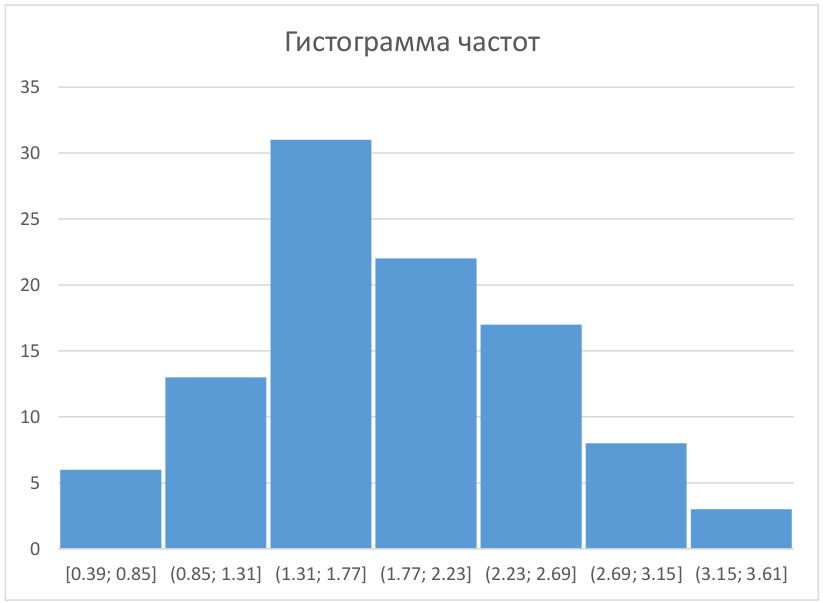
\includegraphics[width=0.9\linewidth]{hist.png}\\
5) Построим дискретный вариационный ряд. Для этого интервалы заменяем их серединами
$\tilde{x_i}$, причем частоты остаются прежними. Рассчитаем точечные оценки для математического ожидания и дисперсии.\\
\begin{tabular}{ | l | l | l | l | l | l | l | l | }
  \hline
  Середины интервалов $\tilde{x_i}$ & 0,62 & 1,08 & 1,54 & 2 & 2,46 & 2,92 & 3,38 \\ \hline
  Частота $n_i$ & 6 & 13 & 31 & 22 & 17 & 8 & 3 \\ \hline
\end{tabular}

Точечной оценкой математического ожидания является выборочная средняя $\bar{x}$
\[
  \bar{x} = \frac{1}{n}\sum_{i=1}^m\tilde{x_i}n_i
\]

\begin{multline}
  \bar{x} = \frac{0.62\times6+1.08\times13+1.54\times31+2\times22+2.46\times17+2.92\times8+3.38\times3}{100}=\\
  =\frac{184.82}{100}=1.8482
\end{multline}
Итак, $\bar{x}=1.8482$

Точечной оценкой дисперсии является несмещённая выборочная дисперсия $s^2$:
\[
  s^2 = \dfrac{\sum_{i=1}^m(\tilde{x_i} - \bar{x})^2n_i}{n-1}
\]
\begin{multline}
  s^2 = \frac{(0.62-1.8482)^2\times6
  + (1.08-1.8482)^2\times13+(1.54-1.8482)^2\times31}{99}+\\
  + \frac{(2-1.8482)^2\times22+(2.46-1.8482)^2\times17+(2.92-1.8482)^2\times8}{99}+\\
  +\frac{(3.38-1.8482)^2\times3}{99} =\frac{42.766}{99}=0.4320
\end{multline}
Несмещённое среднее квадратическое отклонение:
\[
  s= \sqrt{s^2} \approx 0.6573
\]
6) Анализируя результаты исследования, гистограмму распределения, можно
предположить, что данная выборка (масса одного колоса пшеницы сорта \textit{Sonnora})
имеет нормальное распределение со средней массой одного колоса примерно 1.85г
и средним квадратическим отклонением $0.6573$г.

\section{Задача}
\underline{Условие:} Построить 90\%-ный доверительный интервал для вероятности
попадания снаряда в цель, если после 220-ти выстрелов в цель попало 75 снарядов
(предполагается, что случайная величина - попадания снаряда в цель - имеет
нормальное распределение).

\end{document}

% EOF
